%!TEX program = xelatex
\documentclass[12pt,a4paper]{article}
\usepackage[margin=0in]{geometry}
\setlength{\parindent}{0pt}
\usepackage[dvipsnames,prologue,table]{pstricks}
\usepackage{graphicx}
\usepackage[T1]{fontenc}
\usepackage{lmodern}
\usepackage{pst-text}% http://ctan.org/pkg/pst-text
\usepackage[scaled]{helvet}
\renewcommand*\familydefault{\sfdefault}
% \usepackage{uarial}
% \renewcommand{\familydefault}{\sfdefault}

%R147 G191 B235
\definecolor{fcup}{rgb}{0.57,0.75,0.92}

\usepackage{lipsum}

\usepackage{environ}% http://ctan.org/pkg/environ
\newdimen\fontdim
\newdimen\upperfontdim
\newdimen\lowerfontdim
\newif\ifmoreiterations
\fontdim12pt

\makeatletter
\NewEnviron{fitbox}[2]{% \begin{fitbox}{<width>}{<height>} stuff \end{fitbox}
  \def\buildbox{%
    \setbox0\vbox{\hbox{\minipage{#1}%
      \fontsize{\fontdim}{1.2\fontdim}%
      \selectfont%
      \stuff%
    \endminipage}}%
    \dimen@\ht0
    \advance\dimen@\dp0
  }
  \def\stuff{\BODY}% Store environment body
  \buildbox
  % Compute upper and lower bounds
  \ifdim\dimen@>#2
    \loop
      \fontdim.5\fontdim % Reduce font size by half
      \buildbox
    \ifdim\dimen@>#2 \repeat
    \lowerfontdim\fontdim
    \upperfontdim2\fontdim
    \fontdim1.5\fontdim
  \else
    \loop
      \fontdim2\fontdim % Double font size
      \buildbox
    \ifdim\dimen@<#2 \repeat
    \upperfontdim\fontdim
    \lowerfontdim.5\fontdim
    \fontdim.75\fontdim
  \fi
  % Now try to find the optimum size
  \loop
    %\message{Bounds: \the\lowerfontdim\space
    %         \the\fontdim\space \the\upperfontdim^^J}
    \buildbox
    \ifdim\dimen@>#2
      \moreiterationstrue
      \upperfontdim\fontdim
      \advance\fontdim\lowerfontdim
      \fontdim.5\fontdim
    \else
      \advance\dimen@-#2
      \ifdim\dimen@<10pt
        \lowerfontdim\fontdim
        \advance\fontdim\upperfontdim
        \fontdim.5\fontdim
        \dimen@\upperfontdim
        \advance\dimen@-\lowerfontdim
        \ifdim\dimen@<.2pt
          \moreiterationsfalse
        \else
          \moreiterationstrue
        \fi
      \else
        \moreiterationsfalse
      \fi
    \fi
  \ifmoreiterations \repeat
  \box0% Typeset content
}
\makeatother


%% This code is to make empty letters for the 'PhD's in the corners
\usepackage{stackengine,xcolor}
\newcommand\shadowfy[1]{\expandafter\shadowfypars#1\par\relax\relax}
\long\def\shadowfypars#1\par#2\relax{%
  \ifx#1\relax\else
    \shadowfywords#1 \relax\relax%
  \fi%
  \ifx\relax#2\else\par\shadowfypars#2\relax\fi%
}
\def\shadowfywords#1 #2\relax{%
  \ifx#1\relax\else
    \shadowfyletters#1\relax\relax%
  \fi%
  \ifx\relax#2\else\ \shadowfywords#2\relax\fi%
}
\def\shadowfyletters#1#2\relax{%
  \shadow{#1}%
  \ifx\relax#2\else\shadowfyletters#2\relax\fi}

\newlength\shadowHoffset
\newlength\shadowVoffset
\setlength\shadowHoffset{.2pt}
\setlength\shadowVoffset{.1pt}
\def\primarycolor{white}
\def\secondarycolor{black}

\def\shadow#1{\setstackgap{L}{0pt}\def\stacktype{L}%
  \def\useanchorwidth{T}% CAN BE COMMENTEDD FOR MORE INTERLETTER SPACE.
  \Longstack{%
  \raisebox{0pt}{\textcolor{\primarycolor}{#1}} 
  \kern.7\shadowHoffset\raisebox{.7\shadowVoffset}{\textcolor{\secondarycolor}{#1}}
  \kern-.7\shadowHoffset\raisebox{.7\shadowVoffset}{\textcolor{\secondarycolor}{#1}}
  \kern\shadowHoffset\raisebox{0pt}{\textcolor{\secondarycolor}{#1}}
  \kern-\shadowHoffset\raisebox{0pt}{\textcolor{\secondarycolor}{#1}}
  \kern.7\shadowHoffset\raisebox{-.7\shadowVoffset}{\textcolor{\secondarycolor}{#1}}
  \kern-.7\shadowHoffset\raisebox{-.7\shadowVoffset}{\textcolor{\secondarycolor}{#1}}
  \kern0pt\raisebox{\shadowVoffset}{\textcolor{\secondarycolor}{#1}}
  \kern0pt\raisebox{-\shadowVoffset}{\textcolor{\secondarycolor}{#1}}%
}}



\begin{document}
\thispagestyle{empty}
\psset{unit=1in}
\begin{pspicture}(0,0)(\paperwidth,11.69in)
% \psgrid


\setlength{\fboxsep}{100pt}
\setlength{\fboxrule}{2pt}
\newlength{\xpostitle}
\setlength{\xpostitle}{\paperwidth - 12cm - 215pt}

%%% CHANGE THIS %%%
%% depending on how big the title is,
%% you can shift it up or down by changing the \vpos value
\newlength{\vpos}
\setlength{\vpos}{6in}
\rput[tl](\xpostitle,\vpos){
  % The fontsize of the title adjusts to the 12cm x 12cm box
  \begin{fitbox}{18cm}{6cm}
  %%% CHANGE THIS %%%
  %%% feel free (and encouraged!) to do line breaks ( \\ ) where you want
    \textbf{Obstacle Avoidance \\ Framework \\ based on \\ Reach  Sets}
    % \newline  % add more \newline below to decrease the font size
    % \newline
\end{fitbox}}


\newlength{\xposimg}
\setlength{\xposimg}{\paperwidth - 19cm}
\rput[tl](\xposimg,11){
  %%% CHANGE THIS %%%
  %%% add the image file and adjust the width and the position if you want %%%
  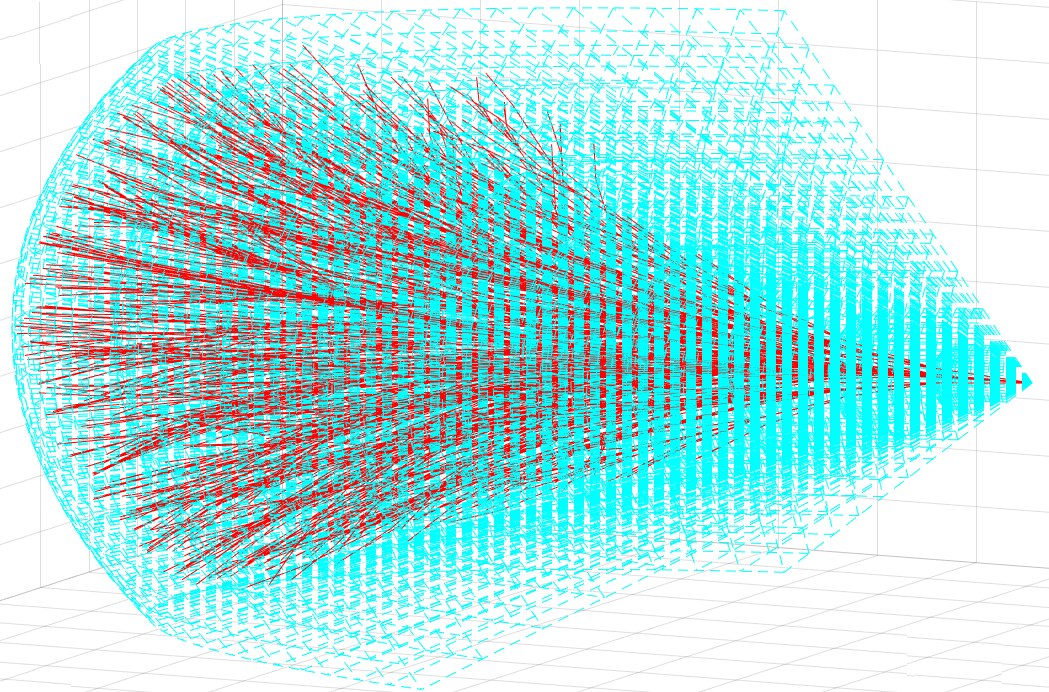
\includegraphics[width=17cm]{placeholder.png}
}




%% depending on how big the title is,
%% you can shift this text up or down by changing the \vpos value
\setlength{\vpos}{2.4in}
\setlength{\xpostitle}{\xpostitle + 0.2cm} %% no idea what the 0.2cm is for...

\rput[Bl](\xpostitle,\vpos){{\fontsize{18pt}{1em}\selectfont %
  %%% CHANGE THIS %%%
  Alojz Gomola
}}

\setlength{\vpos}{\vpos - 1.5em}%
\rput[Bl](\xpostitle,\vpos){{\fontsize{12pt}{1em}\selectfont 
  %%% CHANGE THIS %%%
  Program Doutoral em Matemática Aplicada
}}

\setlength{\vpos}{\vpos - 1.2em}%
\rput[Bl](\xpostitle,\vpos){{\fontsize{10pt}{1em}\selectfont 
  %%% CHANGE THIS %%%
  Departamento Matemática
}}

\setlength{\vpos}{\vpos - 1.2em}%
\rput[Bl](\xpostitle,\vpos){{\fontsize{10pt}{1em}\selectfont 2019}}


\setlength{\vpos}{\vpos - .4in}%
\rput[Bl](\xpostitle,\vpos){{\fontsize{12pt}{1em}\selectfont \textbf{Orientador}}}

\setlength{\vpos}{\vpos - .2in}%
\rput[Bl](\xpostitle,\vpos){{\fontsize{10pt}{1em}\selectfont 
  %%% CHANGE THIS %%%
  João Tasso de Figueiredo Borges de Sousa, DEEC, FEUP
  }}


%%% CHANGE OR REMOVE THIS %%%
\setlength{\vpos}{\vpos - .2in}%
\rput[Bl](\xpostitle,\vpos){{\fontsize{12pt}{1em}\selectfont \textbf{Coorientador}}}

\setlength{\vpos}{\vpos - .2in}%
\rput[Bl](\xpostitle,\vpos){{\fontsize{10pt}{1em}\selectfont 
  %%% CHANGE THIS %%%
  Fernando Manuel Ferreira Lobo Pereira, DEEC, FEUP
  }}


\newlength{\posmiddle}
\setlength{\posmiddle}{\paperwidth / \real{2.0}}




%%% options for the outlined text in the borders
\setlength\shadowHoffset{5pt}
\setlength\shadowVoffset{2pt}
\def\primarycolor{white}
\def\secondarycolor{fcup}

% % top right corner
% \rput[tl]{270}(\paperwidth,11.9){%
%   {\fontsize{215pt}{1em}\selectfont %
%     \textcolor{fcup}{\shadowfy{PhD}}
%   }
% }
% bottom right corner
\rput[lb]{90}(\paperwidth,-0.2){%
  {\fontsize{215pt}{1em}\selectfont %
    \textcolor{fcup}{\shadowfy{Ph}D}
  }
}
% % bottom left corner
% \rput[lb]{-90}(0, 5.3){%
%   {\fontsize{215pt}{1em}\selectfont %
%     \textcolor{fcup}{\reflectbox{\shadowfy{Ph}D}}
%   }
% }



\end{pspicture}
\end{document}
